\chapter{Preliminaries}\label{chapter:preliminaries}

This chapter gives a qualitative and somewhat quantitative treatment of various scientific ideas 
relevant to space weather research. Section \S~\ref{sec:plasma} discusses space plasmas and their properties, 
\S~\ref{sec:mag} introduces the \emph{magnetosphere}, giving context for chapters \ref{chapter:dst_osa},\ref{chapter:dst_msa}. 
Section \S~\ref{sec:plasmadiff} introduces the plasma diffusion model \ref{eq:fokker} and its simplified 
radial diffusion system \ref{eq:radialDiff} which is used as the underlying physical model for chapter 
\ref{chapter:bayes_diff_chapter}. Section \S~\ref{sec:solar} provides some background about the Sun and 
the solar wind which is the driver for all space weather phenomena, this is used in the solar wind prediction 
task considered in chapter \ref{chapter:pdt}.    

\section{Space Plasma}\label{sec:plasma}

Plasma is ubiquitous throughout the visible Universe, also known as the fourth state of matter 
due to its properties which differentiate it from the conventional gaseous state. Plasma is a 
gas which is composed of roughly equal number of positive and negatively charged particles, this
property is known as charge \emph{quasi-neutrality}. The term quasi-neutral is used because although
the gas has almost equal amount of positive and negative charges, the mixture is electricomagnetically 
active. Due to incomplete charge shielding, long range electromagnetic fields play a big role in the 
dynamics of plasma.

%From classical electrostatics the electric potential of a point charge $q$, is given as

%\begin{equation}
%    \phi(r) = \frac{q}{4\pi\epsilon_0 ||r||_2}
%\end{equation}

%where $r$ is the position in space with respect to the charge and $\epsilon_0$ is the \emph{permitivity} of vacuum.

\subsection*{Debye Length}

In a quasi-neutral plasma, due to the prescence of partial electric shielding the potential due to the charges
now takes the so called Debye form.
\begin{equation}
    \phi(r) = \frac{q}{4\pi\epsilon_0 r} e^{-\frac{r}{\lambda_d}}
\end{equation}
where $r$ is the spatial distance with respect to the charge and $\epsilon_0$ is the \emph{permitivity} of vacuum.


The electric potential decays with the Debye length scale $\lambda_d$ at which a balance between thermal vibrations 
which can disturb quasi-neutrality and electrostatic forces due to charge separation. The Debye length scale depends
on the electron temperature and plasma density.

\begin{equation}\label{eq:debye}
    \lambda_d = \sqrt{\frac{\epsilon_0 k_b T_e}{n_e e^2}}
\end{equation}

In equation \ref{eq:debye}, the Debye length scale is expressed in terms of the \emph{Boltzmann constant} $k_b$, 
the electron temperature $T_e$, free space permitivity $\epsilon_0$ and electron charge $e$. One can visualise the 
positively charged ions having a cloud of electrons shielding them at the distance of $\lambda_d$. 

It is also possible to take into account the shielding effect of the ions. The effective Debye length is now 
expressed as an addition of two terms, one for electrons (\ref{eq:debye}) and a similar term for the ions by replacing 
$T_e$ for the ion temperature $T_i$ ($n_i \approx n_e$). 

\subsection*{Plasma Parameter}

Consider a Debye sphere of radius $\lambda_d$, this sphere contains $N_e = \frac{4}{3}\pi \lambda^3_d n_e$ electrons. 
The plasma parameter $g$ is defined as $N_{e}^{-1}$. Rewriting this, we can say:

\begin{equation}
    g \sim \sqrt{\frac{n_e}{T_e}}
\end{equation}

~The description of plasma used in many applications in Space is applicable when $g \ll 1$, in this situation 
the Debye shielding is significant and the quasi-neutral plasma obeys collective statistical behaviour. 
The plasma parameter $g$ also correlates with the collision frequency. As the collisions in plasma increase 
with increasing density and decreasing temperature, if $g \longrightarrow 0$ the plasma becomes nearly collisionless. 
The collisionless property helps in making simplfying assumptions about plasma dynamics and is the starting point 
for the \emph{adiabatic} theory of plasma motions in the Earth's magnetosphere which will be discussed in section 
\S~\ref{sec:plasmadiff}.

\section{Sun \& the Solar Wind}\label{sec:solar}

\begin{figure}
    \noindent\centering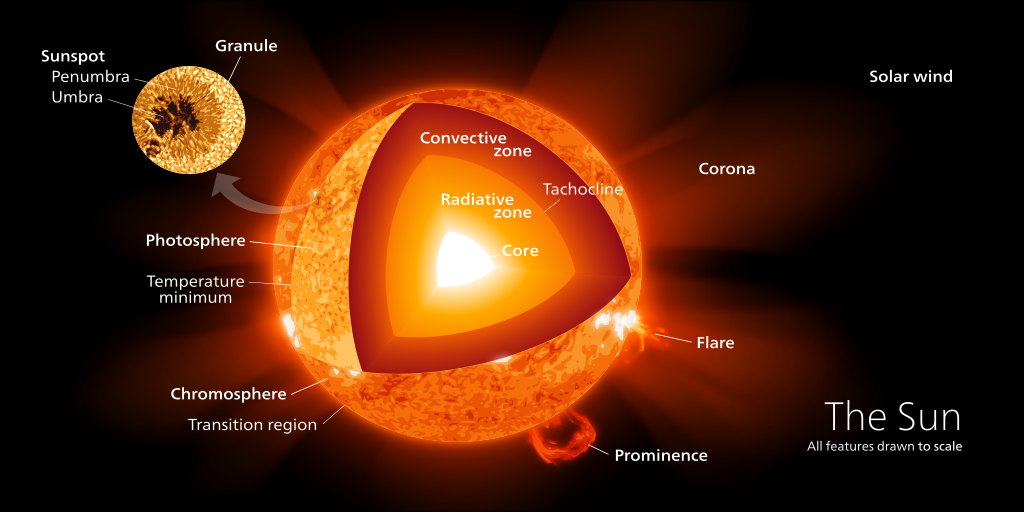
\includegraphics[width=\textwidth]{Sun_poster.png}
    \caption{\small{Cross section of the Sun \\ 
    Author: Kelvinsong [CC BY-SA 3.0 (\url{https://creativecommons.org/licenses/by-sa/3.0})]}}
    \label{fig:SunLayers}
\end{figure}

The Sun is an almost perfectly spherical ball of plasma which is the dominant star in our solar system and 
the principal source of light and energy for all living and meteorological processes on Earth. Apart from 
terrestrial weather, the Sun is also the primary driver of space weather which results from the interaction 
between the solar wind and planetary magnetospheres.

\subsection{Structure}

Figure \ref{fig:SunLayers} shows a cross section of the Sun with various layers. We give a brief description 
of them below.

\textbf{Core}: The core of the Sun is the site for the thermonuclear fusion reactions which produce its energy. 
It extends from the center to about $20-25\%$ of the solar radius \citep{SolarAct}. It has a temperature close to 
$1.57 \times 10^7$ Kelvin and a density of $150 \text{g}/\text{cm}^3$ \citep{SolarCore}. Nuclear fusion in the core 
takes place via the so called \emph{proton-proton chain} (pp).

\textbf{Radiative Zone}: The radiative zone extends from $25\%$ to $70\%$ of the solar radius. The nuclear reactions 
in the core are highly sensitive to temperature and pressure, in fact they are almost shut off at the edge of the core. 
In the radiative zone, energy transfer takes place via photons (radiation) which bounce around nuclei until 
they reach the Convective zone.

\textbf{Convective Zone}: Between $70\%$ of the solar radius to a point close to the solar surface. Density decreases 
dramatically going from the core to the radiative and subsequently the convective zone. Here the solar material behaves more 
like a fluid. Due to the temperature gradient which exists across it, the primary source of transport is 
via convection.

\textbf{Photosphere}: The photosphere is the visible 'surface' of the Sun, since the layers below it are all opaque to 
visible light.A layer of about $100$ kilometre thickness, the photosphere is also the region from where sunlight can freely 
escape into space. The photospheric surface has a number of features i.e. sunspots, granules and faculae. 
Sunspots (see section\S~\ref{sec:sunspots}) are magnetic regions where the solar material has lower temperature as compared 
to its surroundings. Magnetic field lines are concentrated in sunspot regions and the field strength in sunspots can often 
be thousands of times stronger than the on the Earth.

% \begin{wrapfigure}{r}{0.4\textwidth}
%     \centering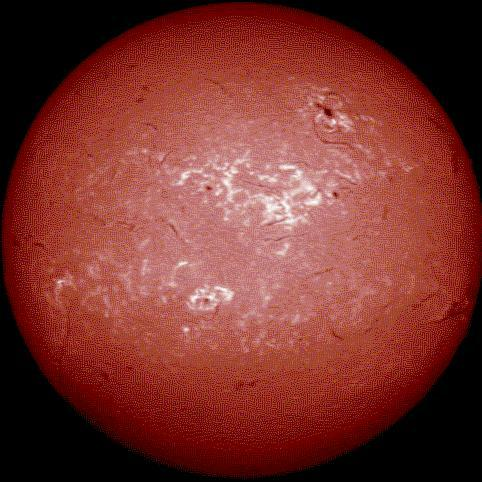
\includegraphics[width=0.38\textwidth]{chromosphere.jpg}
%     \caption{
%         \small{Chromosphere viewed using an $H\alpha$ filter. \\ \textit{Source}: CWitte (Public domain)}}
%     \label{fig:chromosphere}
% \end{wrapfigure}


\textbf{Chromosphere}: Extending for a distance of almost $5000$ kilometers after the photosphere. The chromosphere is 
known for the existense of features called \emph{spicules} and prominences. The chromosphere has a red colour which 
is generally not visible due to the intense light given off by the photosphere, but can be observed through 
a filter centered on the Hydrogen $H\alpha$ spectral line. %(see figure \ref{fig:chromosphere}). 

\textbf{Solar Transition Region}: A thin ($100 \text{km}$) region between the chromosphere and the solar corona 
where the temperature rises from about $8000 \text{K}$ to $500000 \text{K}$. The transition region might not be well 
defined at all altitudes, but its existence is evidenced by a bifurcation of the dynamics of the solar plasma. 
Below the transition region, the dynamics is dictated by gas pressure, fluid dynamics and gravitation while 
above the region the dynamics is dictated more by magnetic forces.

\textbf{Corona}: An aura of plasma around the Sun that extends millions of kilometers into space, the corona can be 
observed during a total solar eclipse or with a coronograph. The temperature of the corona is dramatically higher 
than the photosphere and chromosphere. The average temperature can range between 
$1 \times 10^6 \ \text{to} \ 2 \times 10^6 \text{K}$ while in the hottest regions it can be as high as 
$2 \times 10^7 \text{K}$ \citep{SolarCorona}. Although the reason for this dramatic increase is still 
not well understood, there various explanations using concepts of magnetic reconnection 
\citep{russell2001solar,SolarCorona} and Alfv\'en waves \citep{AlfvenCorona}.


\subsection{Heliospheric Magnetic Field \& Solar Wind}

The existence of the solar wind was first postulated via observations of Halley's coment in 
\citet{Bierman1,Bierman2,Bierman3} and subsequently models of the \emph{Heliospheric Magnetic Field} (HMF) 
were introduced in \citet{parker1958dynamics}. These models were further evidenced by their ability 
to explain the effect of the HMF on the modulation of galactic cosmic rays and their measured intensities 
close to the Earth \citep{ParkerSolarWind}. The structure of the HMF is central to explaining 
the formation and propagation of the solar wind. 

The HMF in steady state points radially outward and rotates with the Sun, producing an \emph{Archimedian spiral} 
structure as postulated in \cite{parker1958dynamics} and shown schematically in figure \ref{fig:parkerspiral}. 
Photospheric observations of the magnetic field (see Global Oscillation Network Group \url{https://gong.nso.edu}) 
are often extrapolated to compute approximations to the HMF. There exist a number of models used to perform such 
extrapolations, such as the \emph{Potential-Field Source Surface} model (PFSS) 
\citep{schatten1969model,altschuler1969magnetic}, the \emph{Current-Sheet Source Surface} model (CSSS) 
\citep{csss} and the \emph{Magnetohydrodynamics Around a Sphere} model (MAS) 
\citep{linker1999magnetohydrodynamic}. 

The HMF can be seen as a combination of two components: the poloidal magnetic field and the toroidal magnetic field.
The two fields often exchange energy between themselves over the course of several years in a cyclical phenomenon
known as the \emph{solar cycle} (section \S~\ref{sec:sunspots}). Interested readers can read \citep{Owens2013} for an 
in-depth review on the phenomena that drive the HMF.
\todo{\textbf{TODO}: Check that the HMF image can be reproduced here.}

\begin{figure}
    \noindent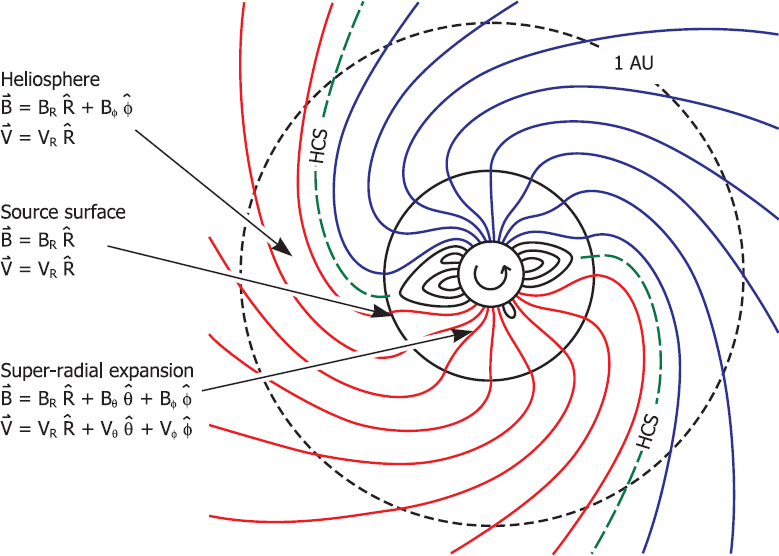
\includegraphics[width=0.8\textwidth]{parker-spiral.jpg}
    \caption{\small{An illustration of the Heliospheric Magnetic Field in the \emph{ecliptic plane}. 
    In the heliosphere, rotation of the HMF footpoints within a radial solar wind flow generates an azimuthal 
    component of the HMF, $B_{\phi}$, leading to a spiral geometry. Red and blue lines, 
    showing regions of opposite polarity, are separated by the heliospheric current sheet (HCS), 
    shown as the green dashed line.
    Image reproduced from \citet{Owens2013}}}
    \label{fig:parkerspiral}
\end{figure}


The expansion of the coronal magnetic field leads to an eventual opening of field lines at the source surface 
(see figure \ref{fig:parkerspiral}) and the ejection of the solar wind. This hot plasma consists mostly of protons, 
electrons and a small number of helium and heavy ions. The solar wind spirals outwards in all directions, carrying 
with it the magnetic field. Upon reaching a distance of $1 \text{AU}$ (close to the Earth's magnetosphere), this wind 
has a nominal speed of about $400 \text{km}/\text{s}$ while its high speed component has an average velocity of 
$\sim 700 \text{km}/\text{s}$ (figure \ref{fig:solarwinddist}).

\begin{figure}
    \noindent\centering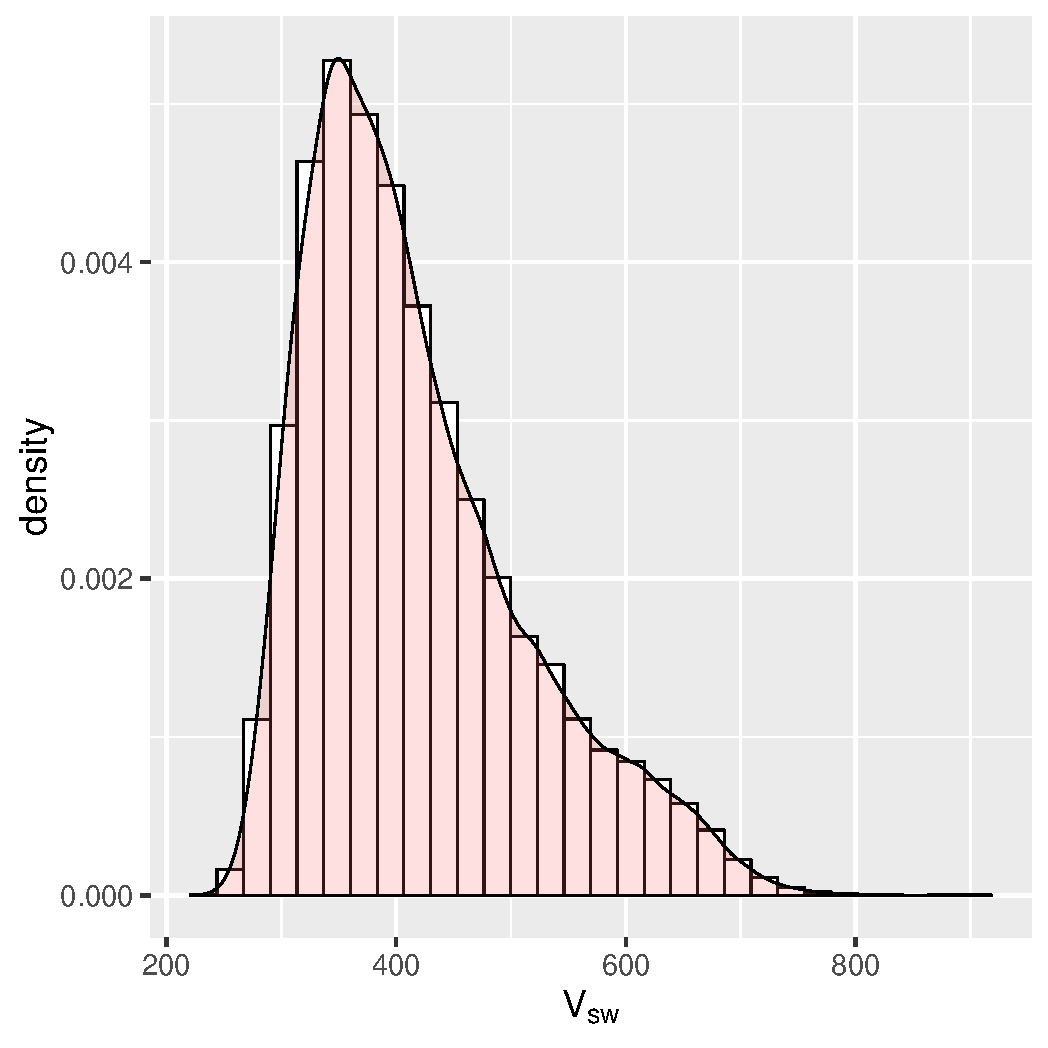
\includegraphics[width=0.75\textwidth]{solarwinddist.pdf}
    \caption{
        \small{Distribution of solar wind speed recorded at 1 AU for the time period $2008 - 2018$}}
    \label{fig:solarwinddist}
\end{figure}

\subsubsection*{Near Earth Measurements}

The solar wind has the heliospheric magnetic field \emph{frozen in} and as it propagates in the interplanetary medium 
it carries the solar magnetic field with it. Important solar wind quantities such as 
\begin{enumerate*} \item solar wind speed \item proton density \item magnetic field strength \end{enumerate*} are recorded 
at the so called $L1$ \emph{Langrangian point} where the gravitational fields of the Earth and the Sun 
approximately balance out.



\subsection{Sunspots \& Solar Cycle}\label{sec:sunspots}

Sunspots are temporarily occuring regions on the Sun's photosphere which appear as dark spots. They are areas 
of magnetic field concentration where the field lines often 'puncture' the solar surface inhibiting convection 
and producing regions with lower temperature than the surroundings. Sunspots generally last anywhere between a 
few days to a few months, they can occur in pairs or groups and can accompany other phenomena such as 
\emph{coronal loops}, \emph{prominences} and reconnection events.

Since the $19^{\text{th}}$ century the number of sunspots on the Sun's surface have been recorded as the 
\emph{sunspot number} (SSN). Sunspots populations increase and decrease behaving as markers for solar activity levels, 
this cyclical behaviour is called the \emph{sunspot cycle} or \emph{solar cycle} (figure \ref{fig:SolarCycle}). 

\begin{figure}
    \noindent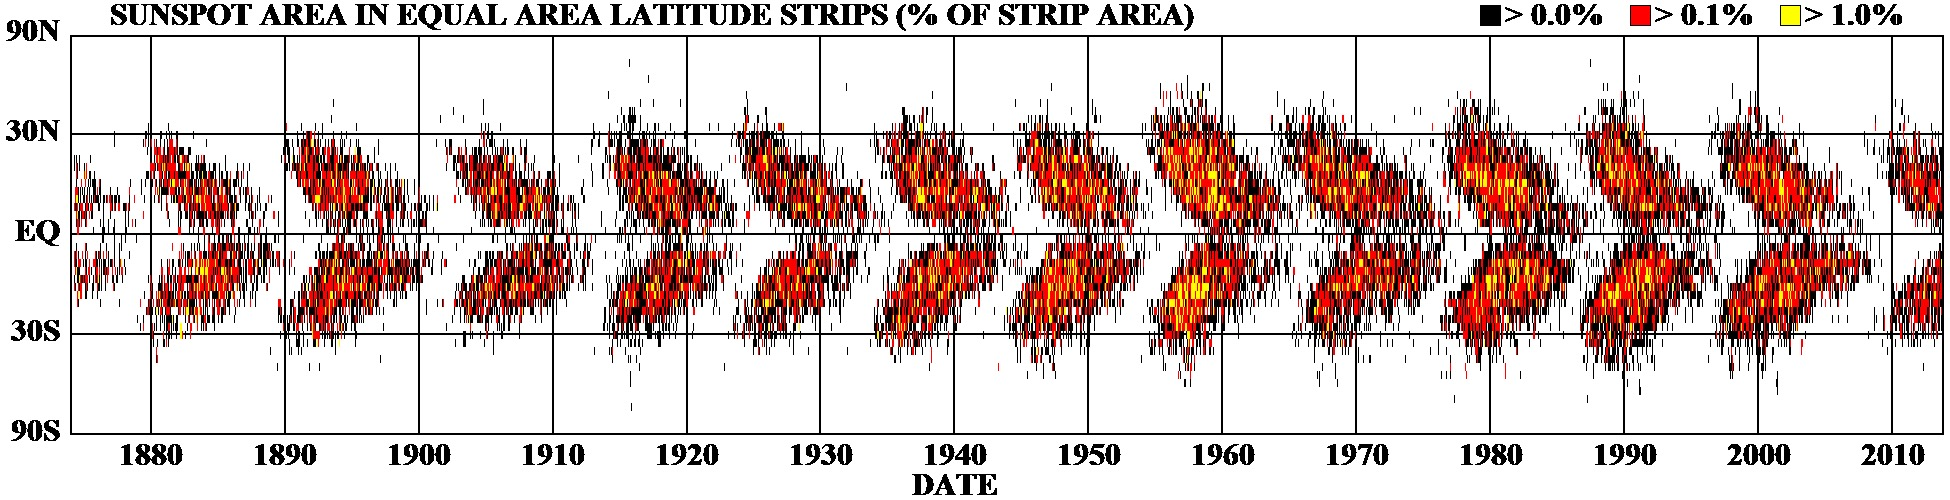
\includegraphics[width=\textwidth]{sunspot-cycle.jpeg}
    \caption{\small{The sunspot butterfly diagram.  \\ 
    Author: David Hathaway, NASA, Marshall Space Flight Center (Public domain) \\ 
    Source: Wikipedia}}
    \label{fig:SolarCycle}
\end{figure}

In figure \ref{fig:SolarCycle} we can see how the area occupied by sunspots changes with solar latitude and time. 
During the start of a solar cycle (solar minimum) sunspots start appearing at higher latitudes, over the course 
of the cycle they move towards the equatorial regions and their number increases to some maximum (solar maximum), 
towards the end the number of sunspots diminishes and the entire cycle starts over. This repetitive behaviour 
happens over approximately $11$ years.

Because sunspots are magnetic phenomena, the solar cycle represents cyclical behaviour of the HMF. During solar 
minimum the poloidal component of the solar magnetic field is at its strongest and it is closest it can get to 
a magnetic dipole configuration. Towards solar maximum energy is transferred from the poloidal component to the 
toroidal component resulting in complex field configurations which are evidenced by larger numbers of sunspot 
clusters.

The solar cycle also gives rise to variations in solar irradiance \citep{solarirradiance}. Between $1645$ and 
$1715$, a period known as the \emph{Maunder minimum} very few sunspots were observed. This coincided with lower 
than average temperatures in Europe, which was called the \emph{little ice age}. Sunspot numbers going back $11000$ 
years have been reconstructed using Carbon-$14$ based analysis of tree rings. Apart from the \emph{Maunder minimum},
other periods of very low sunspot activity have been matched with corresponding \emph{little ice ages}.

In chapter \ref{chapter:pdt}, the \emph{sunspot number} data as well as the \emph{flux tube expansion} factor 
computed by the CSSS model will be used to create a input data set for building the \emph{dynamic time lag regression} 
model proposed therein. Using the input parameters, the DTLR model provides an estimate for the near Earth solar wind speed as 
well as the propagation time. Measurements of the solar wind speed will be used in chapters \ref{chapter:dst_osa}, 
\ref{chapter:dst_msa} as inputs to the forecasting models applied therein.


\section{Magnetosphere}\label{sec:mag}

% \begin{figure}
%     \noindent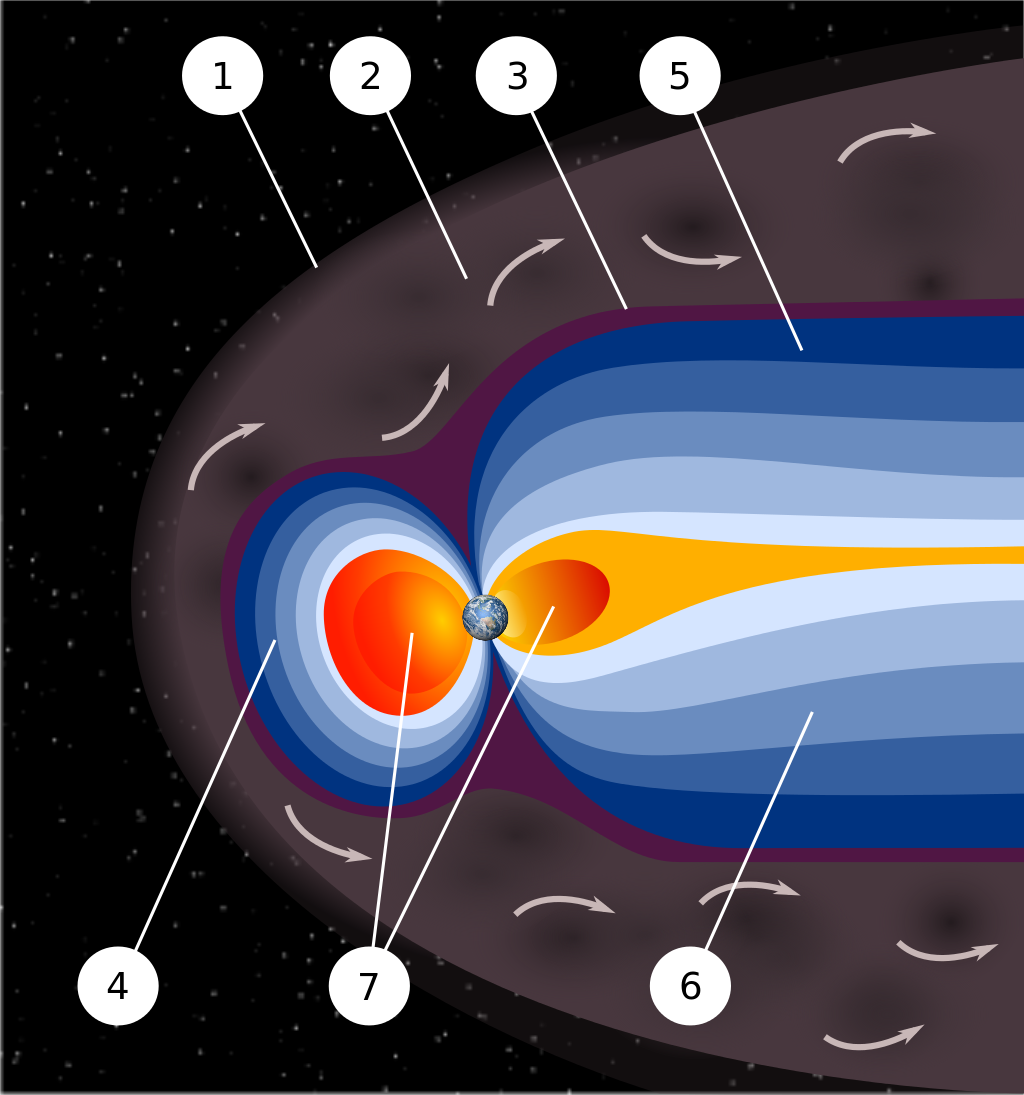
\includegraphics[width=0.7\textwidth]{mag.png}
%     \caption{\small{Schematic diagram of the Earth's magnetosphere: \\
%     The Sun (not shown) is to the left of the figure, the solar wind propagates from left to right.\\
%     1) Bow shock. 2) Magnetosheath. 3) Magnetopause. 4) Magnetosphere. \\
%     5) Northern tail lobe. 6) Southern tail lobe. 7) Plasmasphere.\\ 
%     Source: Dennis Gallagher, derivative work: Fr\'ed\'eric Michel (Public domain)}
%     }
%     \label{fig:magnetosphere}
% \end{figure}

\begin{figure}
    \noindent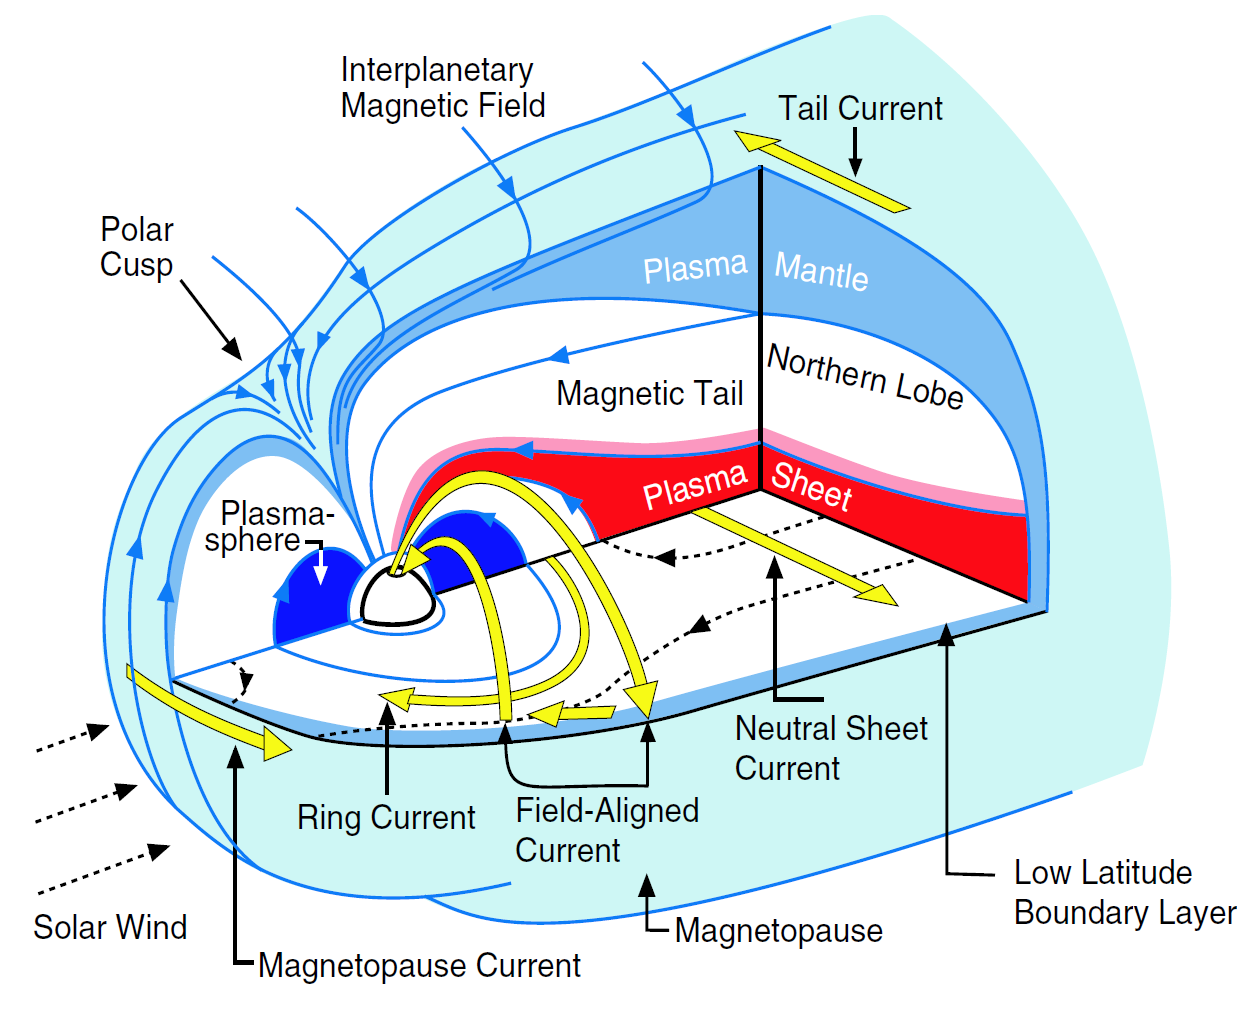
\includegraphics[width=0.8\textwidth]{mag3.png}
    \caption{\small{Three-dimensional cutaway view of the magnetosphere. The light blue outer surface is the magnetopause, 
    its boundary layers are shown in darker blue. Magnetic field lines are shown in blue, electric currents in yellow. 
    The polar region where the magnetic field lines converge is the polar cusp. The bow shock has been omitted for clarity. 
    Reproduced from \citet{DeKeyser2005}}
    }
    \label{fig:magnetosphere}
\end{figure}

The Earth's magnetosphere (figure \ref{fig:magnetosphere}) is a region surrounding the planet where its magnetic field 
dominates the \emph{interplanetary magnetic field}. The Earth's magnetic field shields the atmosphere and terrestrial life 
from the impact of the solar wind. 

As the solar wind approaches the Earth, it is slowed down and deflected by the Earth's magnetic field. Since the 
solar wind is supersonic when it arrives and slows down to subsonic levels, a shock wave is generated in the 
process (\emph{bow shock}). Much of the solar wind kinetic energy is converted to thermal energy when it crosses 
the \emph{bow shock} into the \emph{magnetosheath}. The \emph{magnetosheath} spans from the \emph{bow shock} to 
the \emph{magnetopause}. The \emph{magnetopause} is the outer boundary of the Earth's magnetic shield, its location 
is $\sim 10R_E$ ($R_E = 6372 \text{km}$, the radius of the Earth). 

\begin{wrapfigure}{r}{0.4\textwidth}
    \centering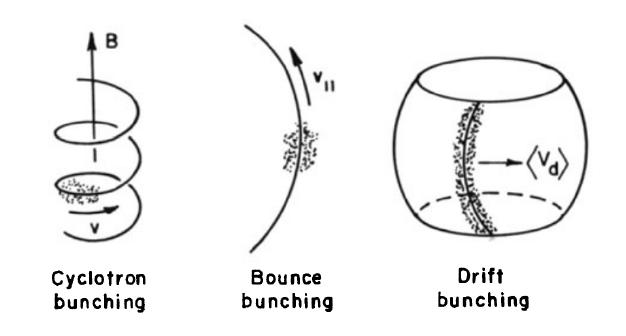
\includegraphics[width=0.35\textwidth]{adiabatic_motions.jpeg}
    \caption{
        \small{Periodic components of particle motion, Reproduced from \citet{roederer2012dynamics}}}
    \label{fig:particlemotions}
\end{wrapfigure}

\todo{\textbf{TODO}: Check that the adiabatic motion image from Roederer can be reproduced here.}

Earth's magnetic shielding is not perfect and some particles manage to get trapped inside the cavity of the 
\emph{magnetosphere}, this region of trapped plasma is known as the \emph{plasmasphere} or the \emph{van Allen 
radiation belts}. Particles trapped in the radiation belts execute complex motions which can be approximately 
modelled using ideas from adiabatic theory and diffusion described in section \S~\ref{sec:plasmadiff} below. 

The portion of the magnetosphere facing away from the Sun (called the \emph{nightside}) is streched out in  
a tail like shape by the deflected solar wind, hence it is referred to as the \emph{magnetotail}. The 
\emph{magnetotail} has an approximate extent of up to $1000R_E$.


\subsection{Particle Motions \& Adiabatic Theory} \label{sec:plasmadiff}

This section gives a quick introduction to the theory of charged particle motions in the magnetosphere, the reader 
may refer to \citet{roederer2012dynamics} for an indepth treatment of this subject.

To understand the motions of charged particles in the \emph{magnetosphere}, the role of electric and magnetic 
forces must be understood.

It is well known from classical electromagnetism that the force exerted on a particle with charge $q$ by a 
magnetic field $\mathbf{B}$ and an electric field $\mathbf{E}$ is given by the so called \emph{Lorentz force} 
(eq \ref{eq:lorentzforce}).

\begin{equation}\label{eq:lorentzforce}
    \mathbf{F} = m\frac{d\mathbf{v}}{dt} = q\mathbf{E} + q\mathbf{v} \times \mathbf{B}
\end{equation}


The first component of equation \ref{eq:lorentzforce} ($q\mathbf{E}$) is either parallel or opposite to the local electric 
field depending on the charge of the particle. The second component $q\mathbf{v} \times \mathbf{B}$ involves a vector 
cross product so it is always perpendicular to the plane spanned by vectors $\mathbf{v}$ and $\mathbf{B}$. In order to 
understand its effects, we can decompose the particle velocity in two components; $v_{\parallel}$ parallel to $\mathbf{B}$ and 
$v_{\perp}$ perpendicular to $\mathbf{B}$. If $\mathbf{E} = \mathbf{0}$, then the particle executes a circular motion 
whose properties are shown in equation \ref{eq:larmor}, $\rho$ is the gyroradius and $\omega$ is the gyrofrequency or 
cyclotron frequency. In case $v_{\parallel} \neq 0$ then the trajectory is helical.

\begin{equation}\label{eq:larmor}
    \frac{v^{2}_{\perp}}{\rho} = \frac{qBv_{\perp}}{m} = \omega v_{\perp}
\end{equation}

Apart from the gyro motion, there are some important drift forces which significantly influence particle motions.

\begin{itemize}
    \item Electric field drift: If $\mathbf{E}$ has a component $E_{\perp}$ perpendicular to $\mathbf{B}$, the electric 
    field accelerates and decelerates the particle in the two hemispheres of the orbit. The orbit becomes 
    a distorted circle and the particle drifts in a direction perpendicular to the electric field with a velocity 
    $\mathbf{v_d} = \mathbf{E} \times \mathbf{B} / B^2$.

    \item Magnetic gradient drift: When the magnetic field varies in space (as is the case of the Earth), a 
    gradient in the field strength in the direction perpendicular to $\mathbf{B}$ gives rise to gradient 
    drift velocity given by $\mathbf{v_g} = \frac{1}{2} m v^2_{\perp}\mathbf{B} \times \frac{\nabla \mathbf{B}}{aB^3}$.

    \item Magnetic curvature drift: If the magnetic field has a curvature then this creates an additional 
    drift motion with velocity $\mathbf{v_c} = \frac{ m v_{\parallel} 
    \mathbf{B} \times (\hat{\mathbf{b}} \cdot \nabla) \hat{\mathbf{b}} }{qB^2}, 
    \ \ \mathbf{b} = \frac{\mathbf{B}}{B}$
\end{itemize}

The equations of motion for charged particles in the general case of spatially varying electric and magnetic fields 
do not admit closed form solutions. The motions are generally complex and require lengthy numerical integrations 
to be resolved.

The \emph{guiding center} approximation helps us to decompose particle motions into three periodic components, 
each with its own time scale (figure \ref{fig:particlemotions}).
\begin{enumerate*}
    \item Gyromotion around magnetic field lines.
    \item Bounce motions between magnetic north and south poles.
    \item Equatorial drift of electrons and protons.
\end{enumerate*}

\subsubsection*{Adiabatic Invariants}

When a physical system with periodic motion is varied slowly as compared to the its time period, this 
transformation is can be characterized as \emph{adiabatic}. Formally speaking, for systems which are described by 
Hamiltonian dynamics, we can write the equations of motion in terms of the \emph{cannonical position} $q$, 
the \emph{cannonical momentum} $p$, external parameters $\theta$ and the system's \emph{Hamiltonian} 
$\mathcal{H}(q,p|\theta)$. 

\begin{align}\label{eq:hamilton}
    \dot q &= \frac{\partial \mathcal{H}}{\partial p}\\
    \dot p &= - \frac{\partial \mathcal{H}}{\partial q}
\end{align}

If the hamiltonian system shown in equation \ref{eq:hamilton} executes a periodic motion in the $q,p$ phase space, 
then it admits an \emph{adiabatic invariant} $A$ given in equation \ref{eq:adiabatic_invariant}.

\begin{equation}\label{eq:adiabatic_invariant}
    A = \oint p dq
\end{equation}

The quantity $A$ would remain approximately constant if the external parameters $\theta$ were varied adiabatically, 
that is if changes in $\theta$ happen over a time period much greater than the period of oscillation of the system.

Applying this idea to charged particle motion in the \emph{magnetosphere}, it is possible to associate one 
adiabatic invariant with each periodic motion i.e. gyromotion $\mathcal{M}$, bounce $J$ and drift 
$\Phi$ (equation \ref{eq:plasmainv}). 

\begin{align}\label{eq:plasmainv}
    \mathcal{M} &= \frac{1}{2}\frac{mv^{2}_{\perp}}{B} \\
    J &= \oint{m_0 v_{\parallel}ds} \\
    \Phi &= \oint{v_{\text{drift}} \cdot r d\phi} = \int{\mathbf{B} d\mathbf{S}}
\end{align}


The first invariant $\mathcal{M}$ is associated with the Larmor gyration, it is the magnetic moment of the 
current generated by the circular motion of the particle around the field line. 

The second invariant $J$ is associated with the bounce motion between the two magnetic mirrors near the north and 
south poles (the quantity $s$ is an appropriately chosen arc length coordinate along the bounce trajectory). 

The third invariant $\Phi$ associated with the drift motion, is actually the magnetic flux through the barrel 
shape envelope of the particle drift. A particle's guiding magnetic field line can be identified by its radial 
position $r$ and its longitude $\phi$, the magnetic flux of the drift can then be computed by integrating over 
$\phi$.

\subsubsection*{Plasma Diffusion}

Because we consider populations of charged particles, it is natural to employ some kind of distribution based 
picture for magnetospheric plasma. The adiabatic invariants give us a phase space or coordinate system by which 
we can express quantities of interest. 

The main quantity of interest in this case is the \emph{phase space density} $f(t, \mathcal{M}, J, \Phi)$ which 
is a function of time and three invariants. The \emph{phase space density} tells us the number of particles in 
a particular region of the phase space, at a particular point of time.

Diffusion behaviour arises when one or more of the invariants are violated, which can happen due to a number of 
reasons such as: 
\begin{enumerate*}
    \item non-adiabatic variations of the magnetic field 
    \item external forces
    \item interaction with electromagnetic waves
    \item collisions with atmosphere/ionosphere. 
\end{enumerate*}

The plasma diffusion system \citep{schulz2012particle} can be written as a generalized Fokker-Planck system as shown 
in equation \ref{eq:fokker}.

\begin{align}\label{eq:fokker}
    \frac{\partial{f}}{\partial{t}} &= \sum^{3}_{p,q = 1}
    \frac{\partial}{\partial{J_{p}}} \left( \kappa_{pq}
    \frac{\partial{f}}{\partial{J_{q}}} \right) \\
    J_1 &= \mathcal{M} \\
    J_2 &= J \\
    J_{3} &= \Phi
\end{align}

It is possible to simplify this system by considering the two main categories of diffusion, radial diffusion and 
pitch angle diffusion. Radial diffusion allowing particles to move farther or closer to the Earth and pitch angle 
\footnote{pitch angle being the angle between particle velocity $\mathbf{v}$ and the magnetic field $\mathbf{B}$} 
diffusion moving the magnetic mirror points along the field lines.

Rewriting $\Phi \propto \frac{1}{\ell}$, the third invariant can be expressed in terms of the 
\emph{drift shell} $l$ (larger value of $l$ implies greater distance from the Earth). The radial diffusion system 
can be obtained from \ref{eq:fokker} by keeping $\mathcal{M}, J$ fixed, considering diffusion in $\ell$ 
(violation of $\Phi$ invariance) and by approximating pitch angle diffusion as a loss process 
\citep{roederer2012dynamics,Walt1970}.  

\begin{equation}\label{eq:radialDiff}
    \frac{\partial{f}}{\partial{t}} = \ell^2 \frac{\partial}{\partial{\ell}} \left( \frac{\kappa(\ell,
        t)}{\ell^{2}} \frac{\partial{f}}{\partial{\ell}}
    \right)_{\mathcal{M}, J} - \lambda(\ell,t) f
\end{equation}

The resulting system is shown in \ref{eq:radialDiff}, the term 
$\ell^2 \frac{\partial}{\partial{\ell}} \left( \frac{\kappa(\ell,t)}{\ell^{2}} \frac{\partial{f}}{\partial{\ell}}
\right)_{\mathcal{M}, J}$ models diffusive phenomena in $\Phi$ but it expressed in the drift shell coordinate $\ell$. 
Pitch angle diffusion is approximated using a loss process $\lambda(\ell,t) f$, where $\lambda(\ell,t)$ is the 
\emph{loss rate}, as an alternative it is also possible to express the loss rate as a \emph{loss time scale} 
$\tau(\ell,t) = \frac{1}{\lambda(\ell,t)}$, but in this thesis we will use the former convention.

The radial diffusion system in equation \ref{eq:raddiffusion} is the starting point for chapter 
\ref{chapter:bayes_diff_chapter} where a surrogate model of the phase space density $\hat{f}$ is built to 
perform bayesian inference over the parameters of the diffusion coefficient $\kappa$ and loss rate 
$\lambda$.

\subsection{Current Systems \& Geomagnetic Indices}

As was noted earlier, the solar wind is largely deflected by the Earth's magnetic field but some particles still 
leak into the magnetosphere. This particle injection is governed by the interaction between the magnetic field carried 
by the solar wind and the Earth's magnetic field, also known as \emph{solar wind - magnetosphere coupling} it 
plays a important role in determining space weather conditions in Earth's vicinity. 

Solar wind plasma gets trapped in the Earth's magnetic field at a rate that is modulated by the 
\emph{solar wind - magnetosphere coupling}. The drift motions of charged particles in the magnetosphere 
as discussed in section \S~\ref{sec:mag} lead to many current systems. The prominent current systems 
(pictured in figure \ref{fig:magnetosphere}) are \begin{enumerate*} \item ring current 
\item field aligned current \item tail current \item magnetopause current \end{enumerate*}.  
These current systems induce magnetic fields which interact with the Earth's magnetic field and mutate it. 
When the Earth's magnetic field strength is weakened due to strong ring currents, this leads to 
geomagnetic storm conditions which can have adverse impacts on orbiting satellites and ground based 
infrastructure.

For the purposes of space weather monitoring and forecasting, the state of the magnetosphere and geomagnetic 
phenomena are often represented using proxies known as geomagnetic indices. Geomagnetic indices give us the 
ability to summarize the state of the magnetosphere in terse framework. They are often calculated by averaging 
several ground based measurements of magnetic fluctuations, generally at a cadence of a few hours.

Chapter \ref{chapter:dst_osa} gives a brief introduction to the popular geomagnetic indices and formulates 
\emph{gaussian process} models for producing probabilistic one hour ahead forecasts of the $Dst$ 
index. 

In chapter \ref{chapter:dst_msa}, we augment the $Dst$ model from chapter \ref{chapter:dst_osa} with 
\emph{long short-term memory} (LSTM) networks and obtain five hour ahead forecasts of the $Dst$.



\clearpage

%\bibliographystyle{plainnat}
%\bibliography{references}
